




\fancyhead[C]{Abstract}

Computer software operates as an organized array of specialized tools designed for distinct tasks. Similarly, a game engine constitutes a sophisticated software framework comprising diverse computer graphics components.

In contrast, a game editor empowers users to craft new tools seamlessly integrated with existing robust engines, thereby amplifying functionality and customization opportunities.

This article delves into essential components crucial for a game engine, exploring their underlying mechanisms: graphics rendering, physics simulations, and input handling. By unraveling these interactions within the framework, we uncover the intricate processes that underpin the creation of immersive and dynamic gaming experiences.

\vspace{0.5cm}
\hrule
\vspace{0.5cm}

This paper explores foundational literature informing the development of a game engine architecture, focusing on three critical domains: mathematical frameworks, rendering engines, and C++ software infrastructure.

"Mathematics For Game Developers" by Christopher Tremblay introduces vector mathematics and geometric algorithms pivotal for physics and spatial computations. 

Donald Hearn's "Computer Graphics in C/C++" delves into rendering techniques like rasterization and shading. 

"OpenGL SuperBible" by Jr. Richard S. offers modern OpenGL principles crucial for shader development and GPU-based rendering. 

Additionally, "C++ Primer" by Bjarne Stroustrup guides C++ language features and best practices, shaping the engine's software backbone.

This exploration showcases how these resources collectively contribute to a robust game engine architecture, facilitating core systems like graphics rendering, physics simulations, and input handling, essential for immersive gaming experiences.

\vspace{0.5cm}
\hrule
\vspace{0.5cm}

The thesis project comprises three primary components: an editor, a render engine, and a math engine, collectively forming a framework for game development and computational simulations.

\begin{center}
    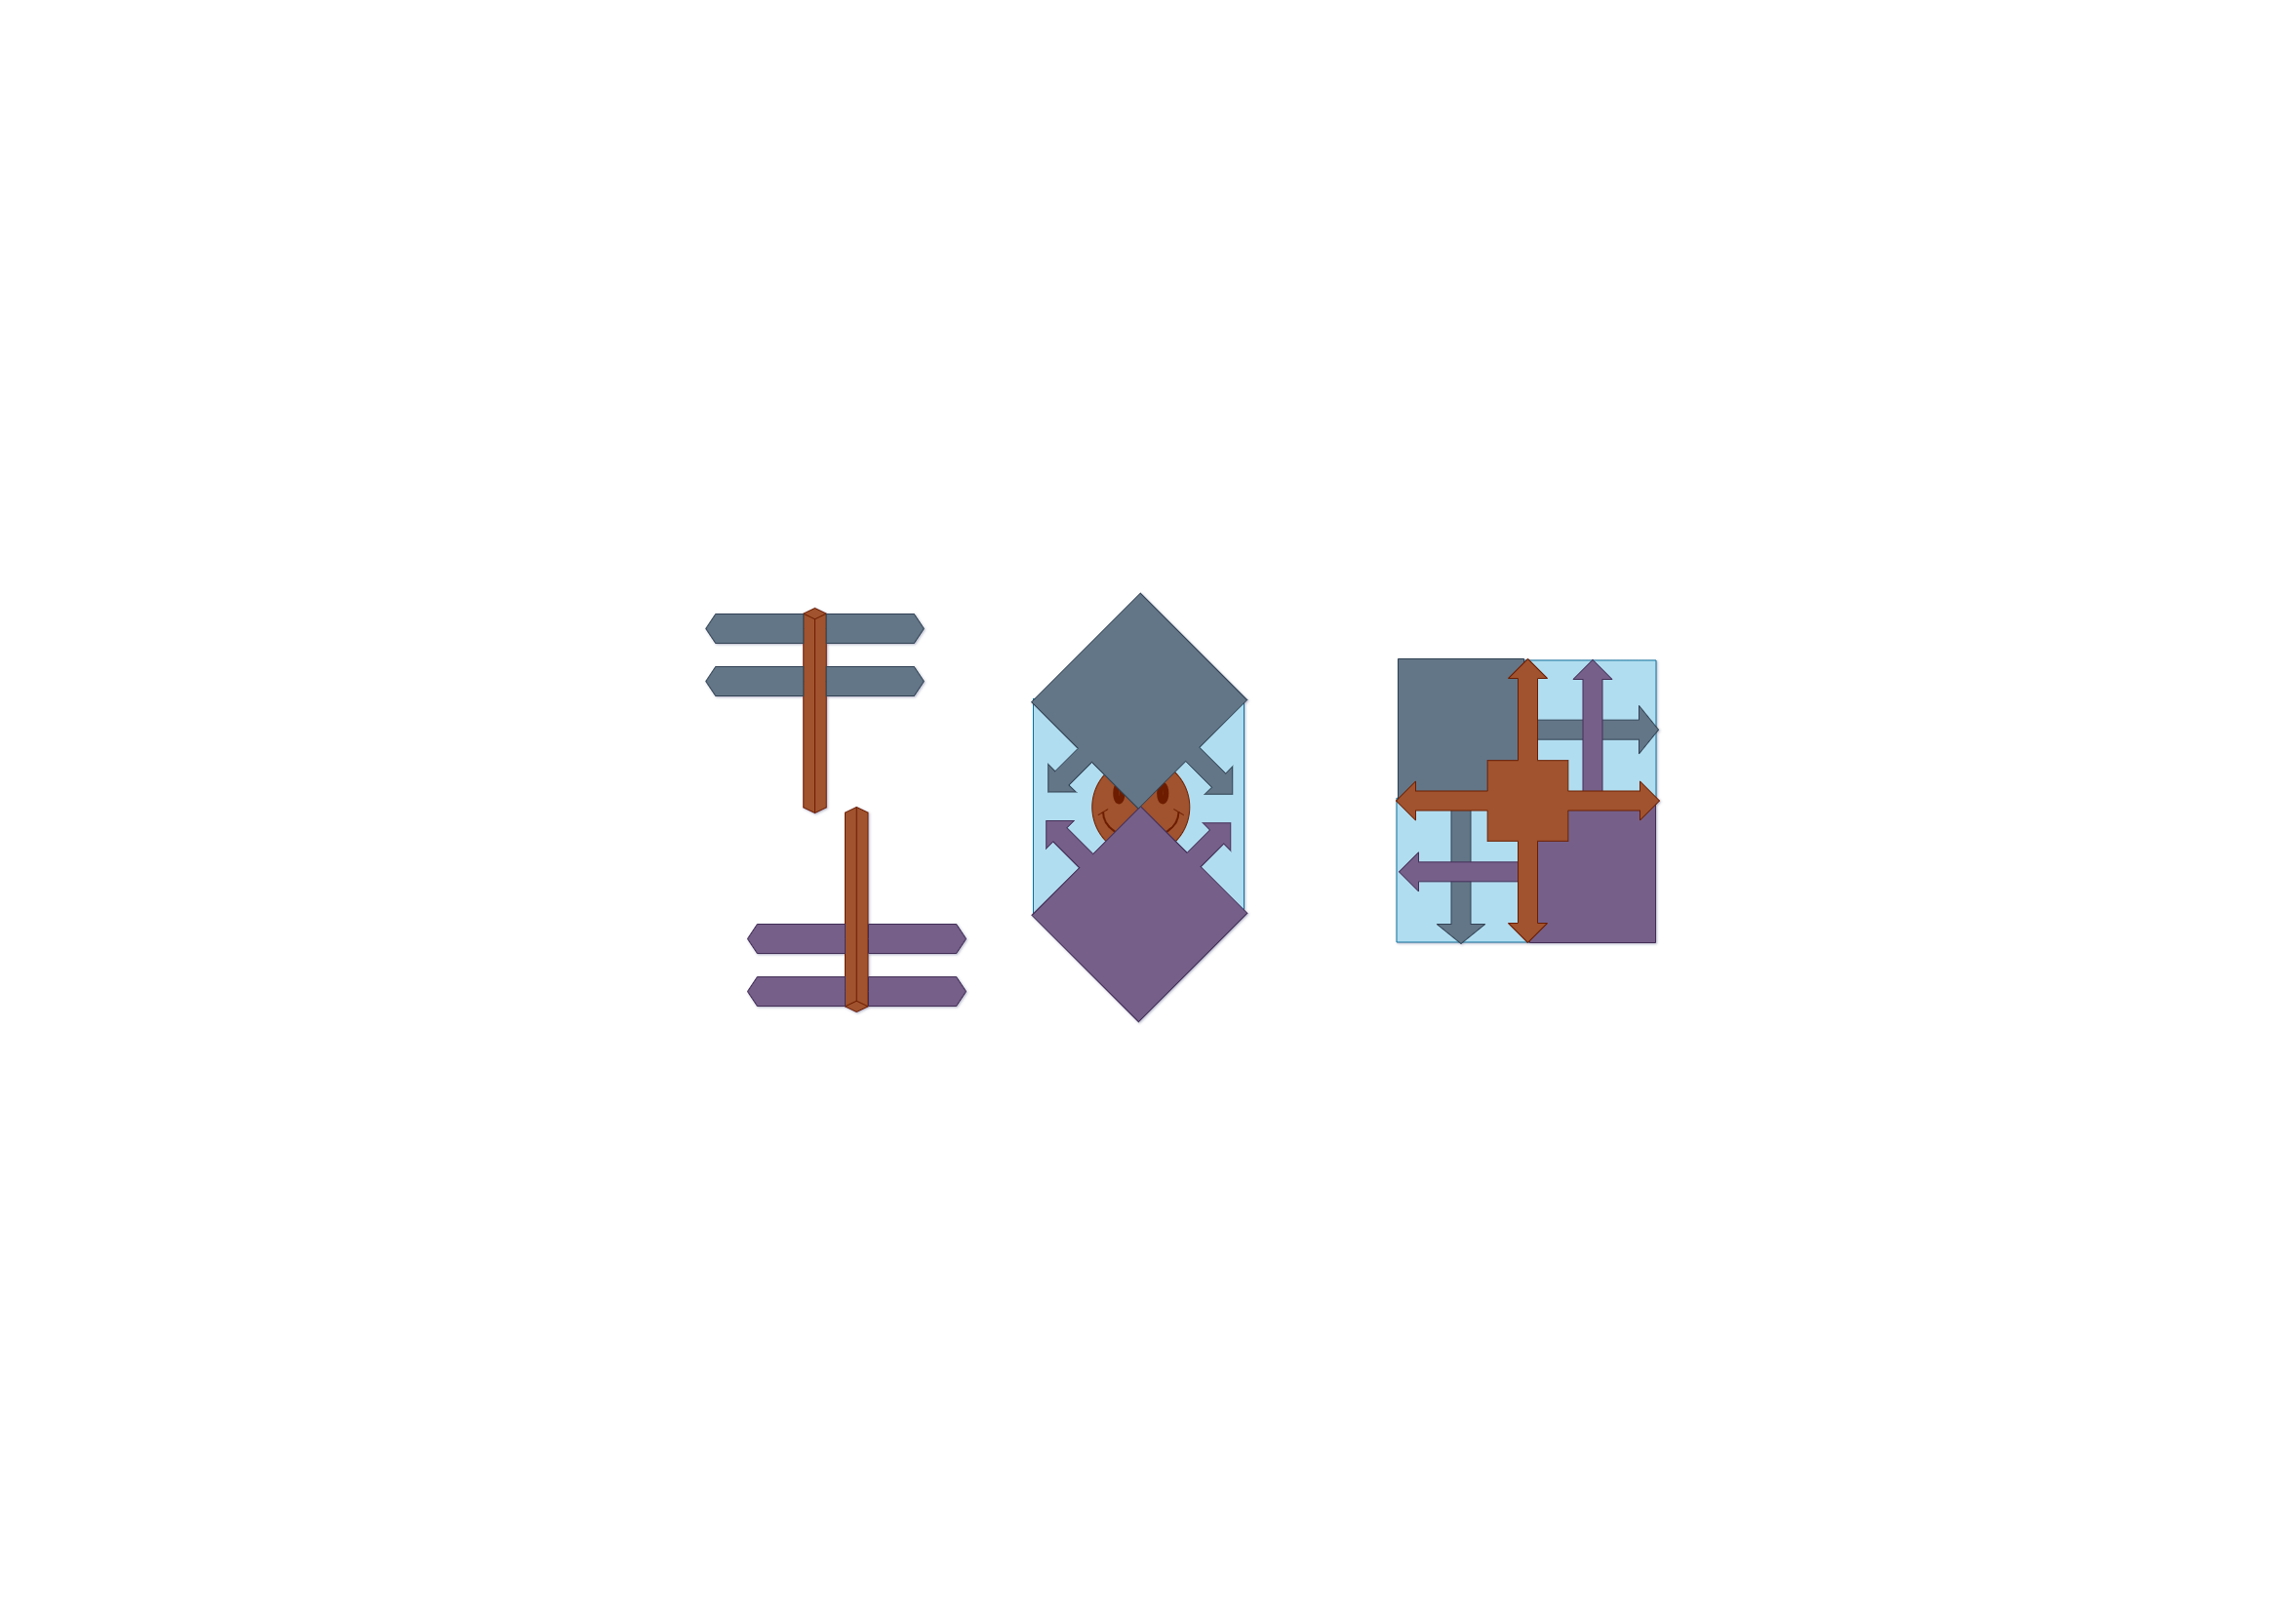
\includegraphics[width=0.7\textwidth]{components.drawio.png}
\end{center}






% \fancyhead[C]{Abstract}




% Computer software operates as an organized array of specialized tools designed for distinct tasks. Similarly, a game engine constitutes a sophisticated software framework comprising diverse computer graphics components.

% In contrast, a game editor empowers users to craft new tools seamlessly integrated with existing robust engines, thereby amplifying functionality and customization opportunities.

% This article delves into essential components crucial for a game engine, exploring their underlying mechanisms. It investigates core systems driving graphics rendering, physics simulations, and input handling. By unraveling these interactions within the framework, we uncover the intricate processes that underpin the creation of immersive and dynamic gaming experiences.

% \hspace{2cm}
% \hrule
% \hspace{4cm}

% This paper explores the foundational literature that informs the development of a comprehensive game engine architecture. Drawing insights from pivotal resources, it organizes knowledge into three distinct domains critical for game engine design: mathematical frameworks, rendering engines, and C++ software infrastructure.

% The "Mathematics For Game Developers" by Christopher Tremblay lays the groundwork with essential vector mathematics and geometric algorithms essential for physics and spatial computations in the game engine. Donald Hearn's "Computer Graphics in C/C++" offers insights into fundamental rendering techniques like rasterization and shading, while Bjarne Stroustrup's "OpenGL SuperBible" provides modern OpenGL programming principles crucial for shader development and GPU-based rendering.

% Furthermore, "C++ Primer" by Bjarne Stroustrup serves as a comprehensive guide to C++ language features, syntax, and best practices, forming the backbone of the game engine's software infrastructure.

% This exploration highlights how these resources collectively contribute to the development of a robust game engine architecture, facilitating the understanding of core systems such as graphics rendering, physics simulations, and input handling. By delving into their inner workings, this paper aims to elucidate the intricate processes essential for creating immersive and dynamic gaming experiences.


% \hspace{2cm}
% \hrule
% \hspace{4cm}

% The thesis project comprises three primary components: an editor, a render engine, and a math engine. These components collectively form a comprehensive framework designed to facilitate game development and computational simulations. 

% \begin{center}
% 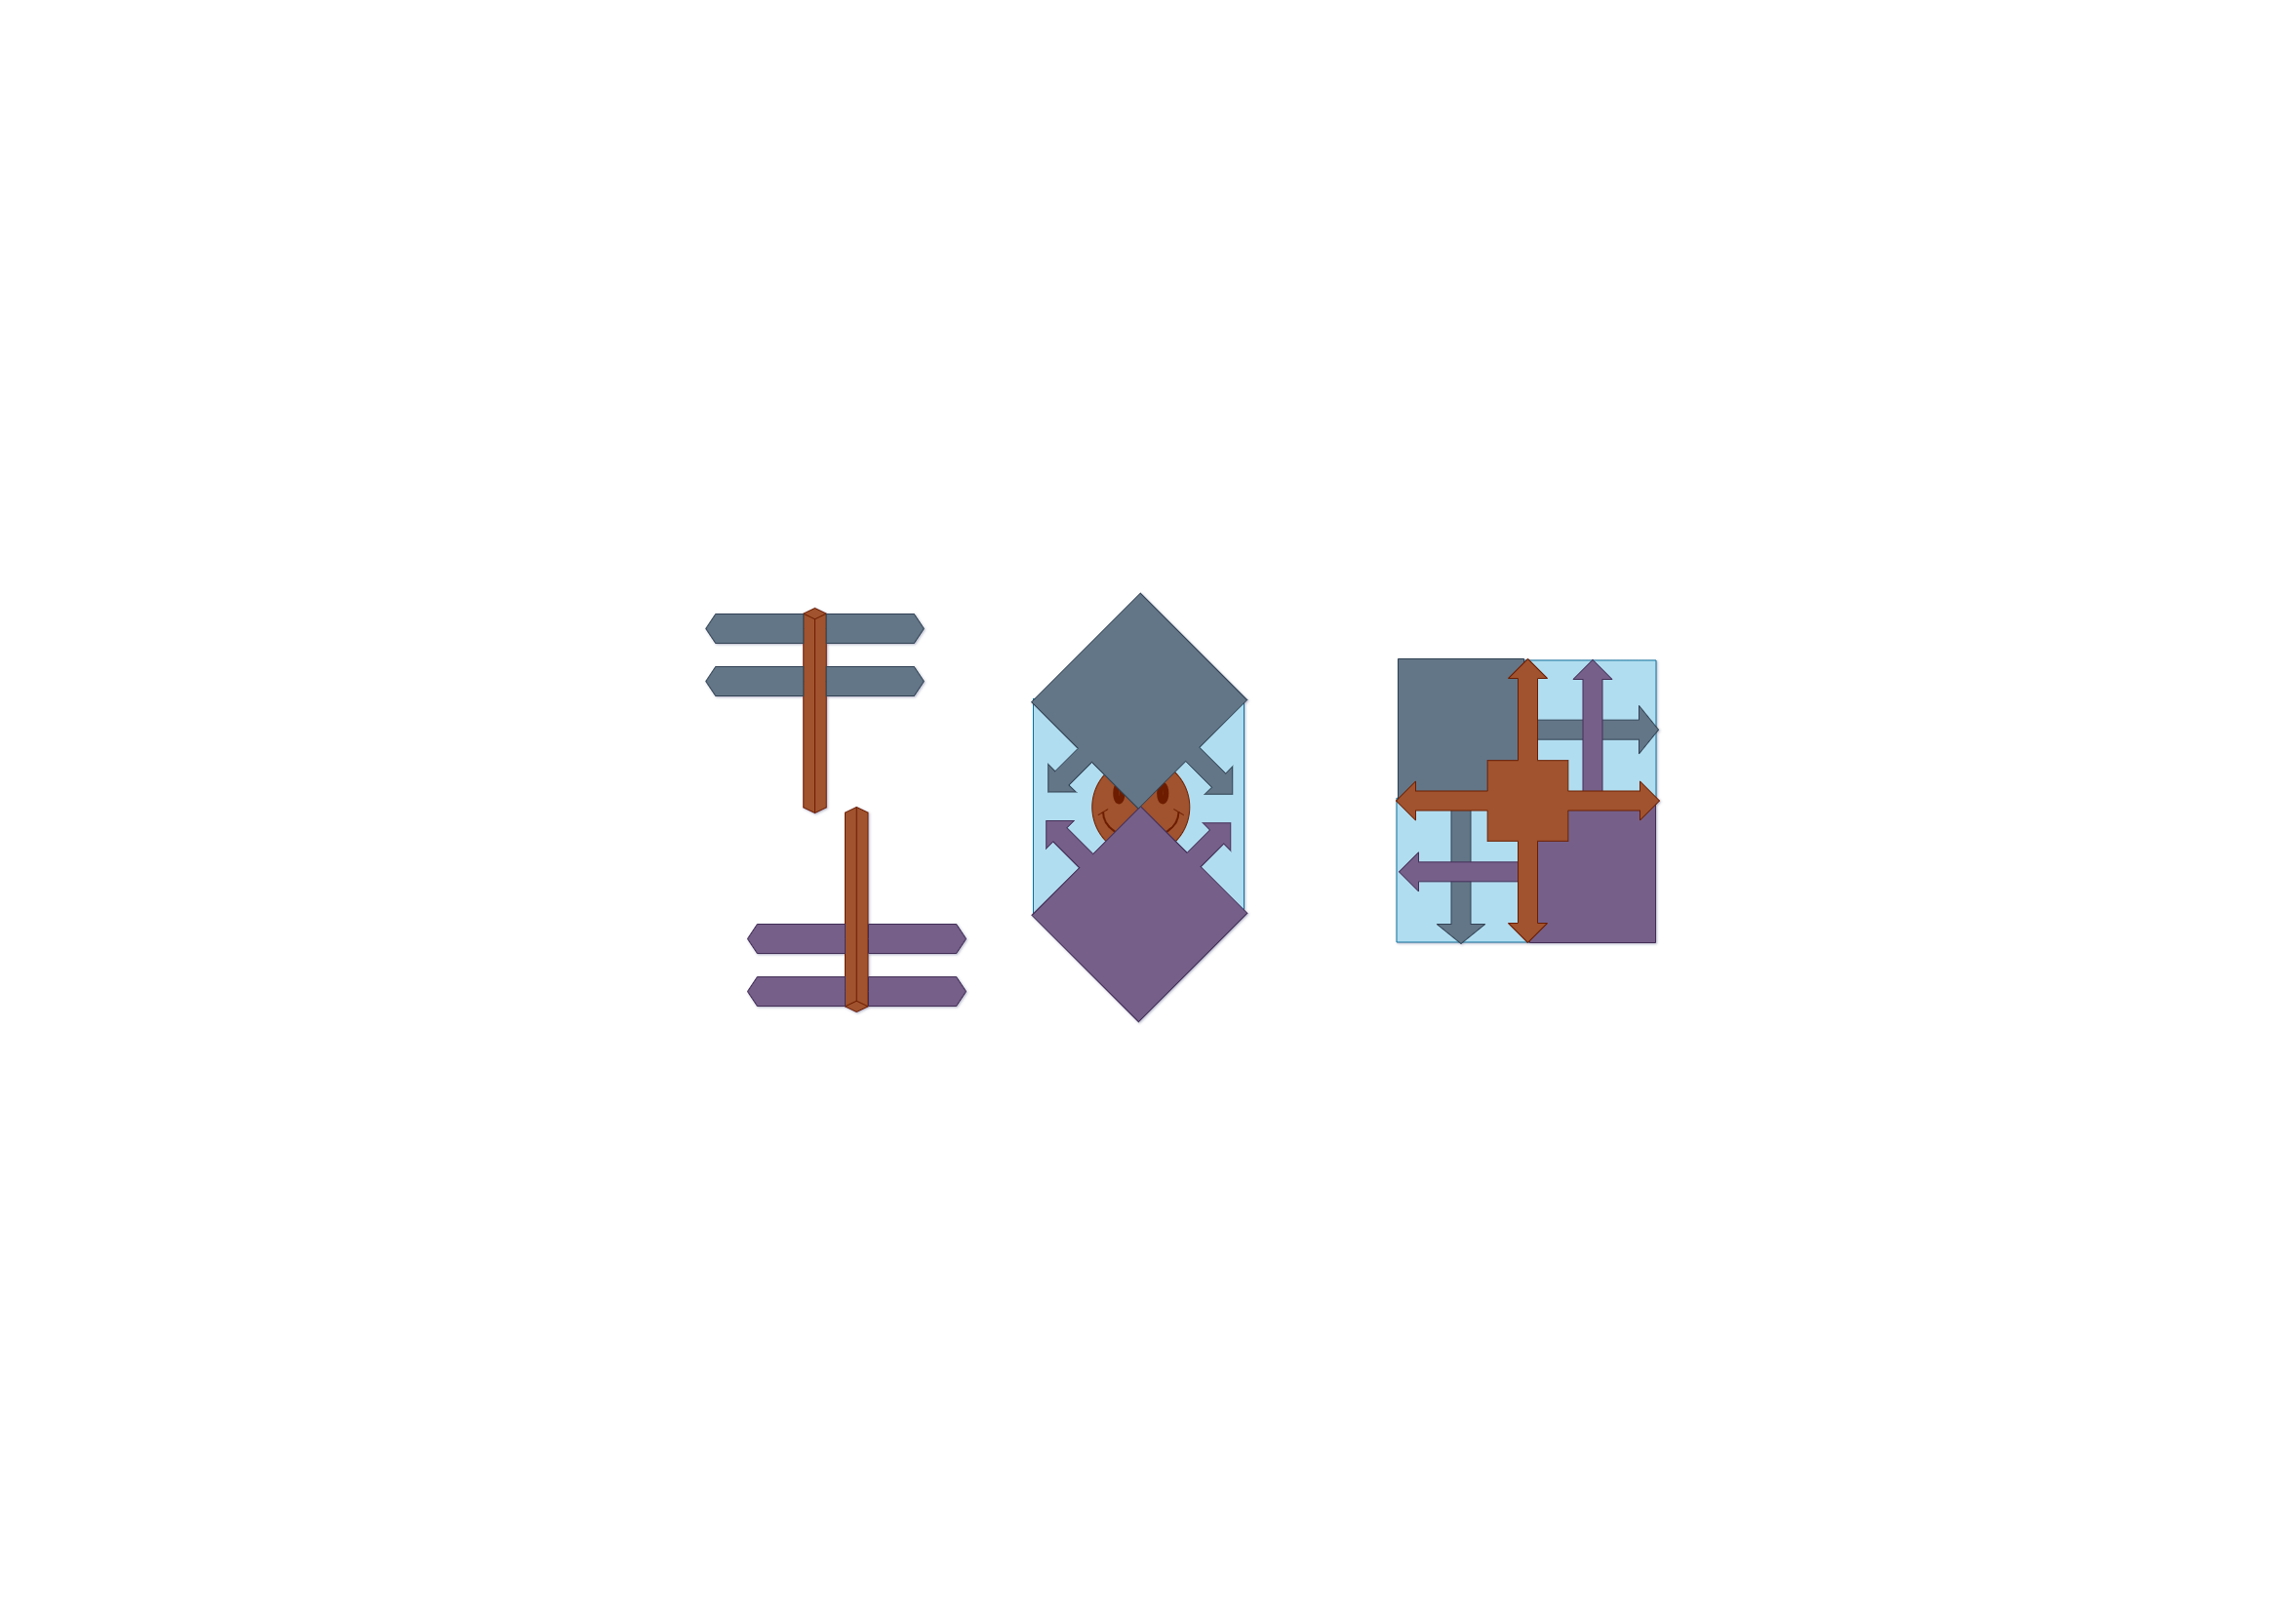
\includegraphics[width=0.5 \textwidth]{components.drawio.png}
% \end{center}


% Computer software can be viewed as a collection of tools meticulously arranged to perform specific functions. In a similar vein, a game engine is a software framework composed of various computer graphics components.

% A game editor, on the other hand, provides users with the capability to create new tools that integrate seamlessly with the existing robust engines, enhancing functionality and customization.

% In the following sections, we will explore the crucial components necessary for a game engine and investigate their inner workings.

%  This exploration will encompass the core systems that drive graphics rendering, physics simulations and input handling. 
% By understanding how these components interact and function within the framework, we can gain insight into the intricate processes that enable the development of immersive and dynamic experiences.



% \begin{center}
% 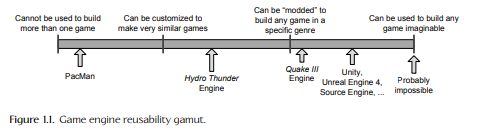
\includegraphics[width=0.9 \textwidth]{game_engine_process.png}
% \end{center}



% \begin{center}
% 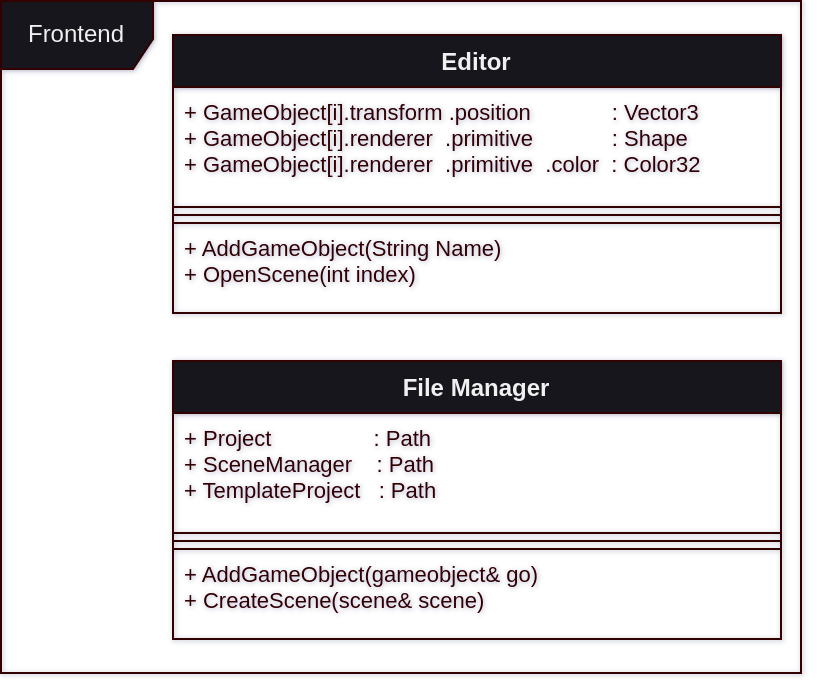
\includegraphics[width=0.486 \textwidth]{app_frontend_overview.png}
% \end{center}


% \begin{center}
% 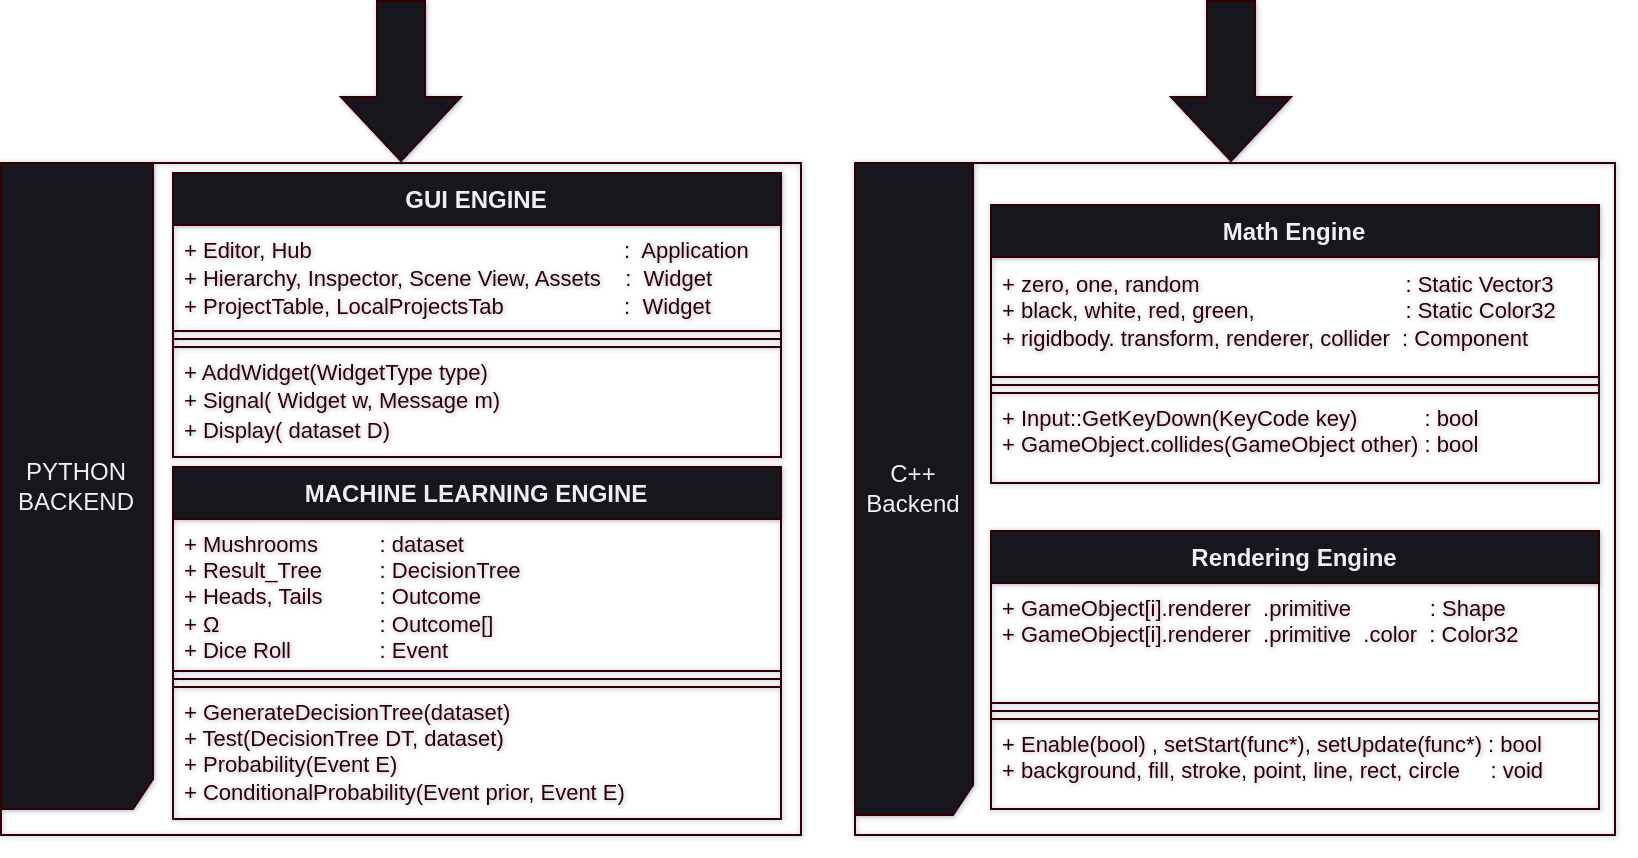
\includegraphics[width=0.9 \textwidth]{app_backend_overview.png}
% \end{center}





% Computer Software is just a bunch of tools orchestrated in just the right manner.


% Similarly to this, a game engine is just a software framework of computer graphics components.


% The Game Editor is what allows users to custom build new tools that work seemingly with the already existing SOLID engines.


